\documentclass[a4paper,11pt,titlepage]{article}

%% %%%%%%%%%%%%%%%%%%%% BEGIN PACKAGES %%%%%%%%%%%%%%%%%%%%

%%\usepackage[top=1in, bottom=1in, left=1in, right=1in]{geometry}

\usepackage{fullpage}
\usepackage{url}
\usepackage{hyperref}
\hypersetup{pdfborder=0 0 0}
\usepackage{graphicx}
\usepackage{subfig}
\usepackage{tikz}
\usetikzlibrary{trees}
\usepackage{amssymb}

%% Linux Libertine
\usepackage[T1]{fontenc}
\usepackage{libertine}
\renewcommand*\oldstylenums[1]{{\fontfamily{fxlj}\selectfont #1}}
\usepackage{libertine}

%% %%%%%%%%%%%%%%%%%%%% END PACKAGES %%%%%%%%%%%%%%%%%%%%


%% %%%%%%%%%%%%%%%%%%%% BEGIN COMMANDS %%%%%%%%%%%%%%%%%%%%

\newcommand{\mailto}[1]{\href{mailto:#1}{\texttt{#1}}}

\let\stdsection\section         % because LaTeX cannot handle
                                % recursive commands
\renewcommand{\section}{\newpage\stdsection}

%% %%%%%%%%%%%%%%%%%%%% END COMMANDS %%%%%%%%%%%%%%%%%%%%


%% Final Report — due: 9th Jan 2012, at 11:00
%% Contents for Final Report: The project report should not be longer than 45 pages, and might be organized according to the following structure:

%% A. High Level, Nontechnical Description Why you should buy this product/listen to this presentation? What is the functionality of the product?
%% B. Short Technical Description
%% Short introduction into technologies used
%% Design of your software, possibly including a diagram of the major components of the project
%% Main achievements
%% C. Software Engineering Issues:
%% What technology was used and why; what other technology was considered but not used and why
%% Any technical challenges encountered and how addressed
%% Any risks anticipated, and how mitigated?
%% Any collaboration/coordination difficulties encountered and how addressed
%% Development and testing methods and/or tools used; comparison of plans with actual achievements
%% Estimates of length of code in each of the components, or any other comparable measure of the effort required.
%% Summary of each team member's contributions
%% D. Validation and Conclusions How did you validate your product? Was the project successful? What did you learn? What might you have done differently?
%% E. Bibliography
%% F. Appendix The appendix is optional, and does not count towards the 45 pages. It may contain thing like: User guide, installation instructions; more extensive design, testing, statistics etc.
%% Feel free to re-use material from the previous reports as you see fit, but make sure that the final report presents a coherent story. Ask advice from your supervisor. You might also draw inspiration from the instructions about writing up your individual project.

%% Bear in mind, that most of the project assessors will not have followed the project throughout and will only have a short time to listen to a presentation or see a demonstration. For this reason they will rely heavily on the report to judge the project.

%% The report should be submitted to SGO in form of a hard copy, as well as electonically through CATE.

\begin{document}
\title{\Huge Visigoth\\\Large Graph visualizations}
\author{
  Andreea-Ingrid Funie\\\mailto{aif109@doc.ic.ac.uk}\and
  Alexandru Scvor\c tov\\\mailto{as10109@doc.ic.ac.uk}\and
  Francesco Mazzoli\\\mailto{fm2209@doc.ic.ac.uk}\and
  Marc-David Haubenstock\\\mailto{mh808@doc.ic.ac.uk}\and
  Maximilian Staudt\\\mailto{ms9109@doc.ic.ac.uk}
}
\date{January 2012}
\maketitle

\begin{abstract}
Visigoth is a tool to generate, analyse and visualise Small World
Networks.  It makes these kinds of networks accessible to anyone new
to their mathematical properties and assists in discovering the
various properties they exhibit by presenting the particular networks
generated by some of the currently published algorithms.
\end{abstract}

\tableofcontents

\section{Introduction}
%% This section corresponds to A in the requirements

\subsection{Realistic looking networks}

\subsubsection{Uses}

\subsubsection{The maths}

\subsection{Small World Networks}

Small World Networks derive their denomination from the well-known
Small World Theorem, which states that any two persons are related
through a chain of at most seven friends.

Indeed, Small Wold Networks are graphs resembling the connections
within human social networks. In other words, they are graphs in which
nodes represent people, and edges between nodes represent relations of
some sort.

For example, if someone were to draw every user of a social network
(e.g. Twitter) on a canvas and then connect each pair of them if they
are registered as “friends” on the platform, the resulting graph is a
Small World Network.  Over the course of time, several mathematical
algorithms that generate random Small World Networks have been
discovered. However, the resulting graphs have only lately begun to
resemble those that have grown naturally in the form of social
networks.

\subsection{Introducing Visigoth}

Visigoth makes peeking into the current state-of-the-art of artificial
Small World Networks simple and fun. By integrating existing
generation algorithms into a single, easy-to-use interface, the user
can make a head start into the small world of Small World Networks,
analyse how these algorithms have evolved over time, see the effects
different algorithm parameters have on the resulting networks, and
compare them to naturally grown networks.

\section{In detail}
%% This section corresponds to B in the requirements

\subsection{Generating Small World Networks}
%% For all of the following, we should include a hand-drawn sketch
%% illustrating the graph generated by the algorithm and an exported
%% image of a large graph Visigoth generated.

\subsubsection{Erdos Renyi}

\subsubsection{Watts Strogatz}

\subsubsection{Bipartite Model}

\subsubsection{Preferential Attachment}

\subsubsection{Real Small World Networks}

\subsection{Visigoth technologies}

\subsubsection{Qt}

\subsubsection{OpenGL}

\subsection{Visigoth graph visualizations}

Cross-platform, efficient, looks-good, user-friendly, easy to develop,
etc.

\section{Engineering Visigoth}
%% This section corresponds to C in the requirements

\subsubsection{Graph drawing algorithms}

Graph drawing is a tricky problem, mainly due to the fact that the prime interest when
engineering one is to please humans' taste, instead of some logical property. A wide array
of such algorithms have been proposed in the history of computer science, and since
drawing graphs is a central task in Visigoth, we had to choose the one that fit best.

First we experimented with the existing solutions. One of the most complete free
graph-drawing algorithm is OpenViz\footnote{\url{http://www.graphviz.org/}}, and it
provides various algorithm:

\begin{itemize}
\item
  \textbf{dot}: A hierarchical layout, used for directed graphs. Our small world networks
  are not directed and it was clear from the beginning that they did not fit this model
  well.

\item
  \textbf{twopi}, \textbf{circo}: Radial and circular layout, respectively. Again,
  unsuitable for the quasi-random networks that we use in Visigoth.

\item
  \textbf{neato}: A spring model layout, which seemed to work reasonably well with random
  graphs.
\end{itemize}

The spring model seemed to be the best fit. This class of algorithm work by treating edges
like springs: in this way clusters of highly connected nodes would be drawn together. To
counter this force (that would lead to nodes lumping together), nodes are treated as
charged particles of the same polarity, causing repulsion between every particle and the
others.

When generating a graph, the particles are first places at random locations in the
space. Then, we apply the algorithm repeatedly until the forces are low enough that we can
consider the graph to be stable.

Spring model algorithms are nice for two reasons:

\begin{itemize}
\item
  Good results: spring force algorithms produce pleasant graphs for almost all kind of
  networks. Some algorithms might produce better results for specific kinds of graph, but
  spring force algorithms are by far the more adaptive.

\item
  Ease of implementation: Our simple implementation of the algorithm take a little less
  then 50 lines of C++ code, and works well up to medium-sized graphs.

\item
  Real time drawing: force based algorithms can be used to show in real time the
  untangling of the graph, which is usually an interesting effect. It also permits
  interaction, for example in the form of node-dragging that changes the shape of the
  graph. We employ both techniques in Visigoth.

\end{itemize}

However, even a simple description of the algorithms reveals its high cost. For each
particle, we need to iterate through all the connected nodes to calculate the spring
forces, and more importantly through all the particles of the graphs to calculate the
repulsion forces. Thus, the algorithm is $O(n^2)$, where $n$ is the number of nodes.

For this reason, our implementation works smoothly up to around a 1000 nodes, but then
performance degrades quickly, and the program becomes unresponsive. Various solutions have
been studied, most of which rely on various approximations.

We chose to implement the FADE algorithm\cite{fade}, which works by recursively
subdividing the graph space into squares, and then treats squares as single particles when
they are far enough. This algorithm, while improving performance, is a lot more complex
then the naive one.

\begin{figure}
  \centering
  \subfloat[Graph view]{
    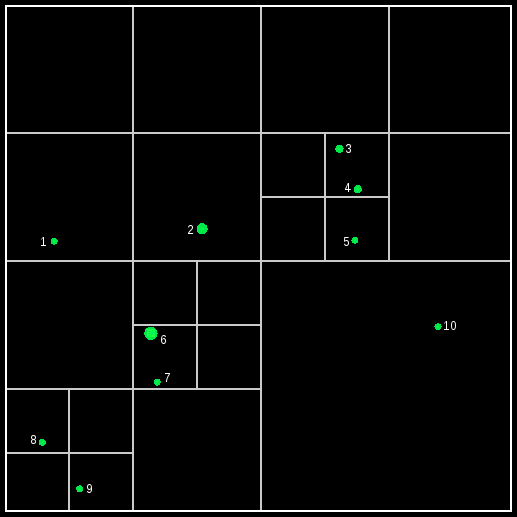
\includegraphics[width=0.4\textwidth]{FADE-quadtree.png}
  }
  \hspace{10pt}
  \subfloat[Tree representation]{
    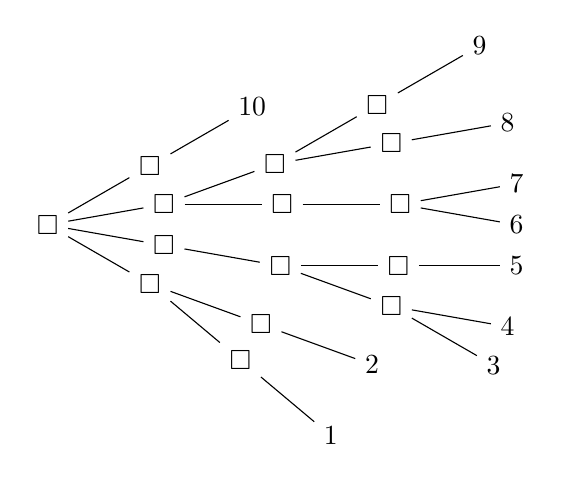
\begin{tikzpicture}[grow cyclic]
      \node {$\square$}
        child {
          node {$\square$}
          child {
            node {$\square$}
            child {node {1}}
          }
          child {
            node {$\square$}
            child {node {2}}
          }
        }
        child {
          node {$\square$}
          child {
            node {$\square$}
                child {
                  node {$\square$}
                  child { node{3} }
                  child { node{4} }
                }
                child {
                  node {$\square$}
                  child {node{5}}
                }
          }
        }
        child {
          node {$\square$}
          child {
            node {$\square$}
            child {
              node {$\square$}
              child {node{6}}
              child {node{7}}
            }
          }
          child {
            node {$\square$}
            child {
              node {$\square$}
              child {node{8}}
            }
            child {
              node {$\square$}
              child {node{9}}
            }
          }
        }
        child {
          node {$\square$}
          child { node {10} }
        }
      ;
    \end{tikzpicture}
  }
  \caption{The QuadTree for a sample graph, empty branches omitted}
  \label{fig:quadtree}
\end{figure}

The first step is to build a data structure representing the recursive subdivision. This
kind of data structure is called a \emph{TreeCode}, which recursively subdivides the space
until only one node remains in the current space, or a maximum depth/minimum space size
size is hit. The space decomposition can be irregular (e.g. \emph{Voronoi} spaces) or
regular. In the latter case, the space is recursively subdivided in squares. We chose to
use a regular, 4-way space decomposition, mainly due to its simplicity. This kind of
structure is called \emph{QuadTree}. Figure \ref{fig:quadtree} shows a sample QuadTree for
a Visigoth graph.

The tree can be built in linear time, and once that is done,

\section{Looking back}
%% This section corresponds to D in the requirements

\subsection{Validation}
%% The client is a happy puppy

\subsection{Lessons learned}

\addcontentsline{toc}{section}{References}
\begin{thebibliography}{9}

\bibitem{hamm10}
  David A. Hammond,
  \emph{Altruism in Small World Models}.
  Imperial College London,
  2010.

\bibitem{oconn11}
  Luke M. O’Connor,
  \emph{Algorithms for Constructing Realistic Networks}.
  Imperial College London,
  2011.

\bibitem{fade}
  Aaron Quigley and Peter Eades,
  \emph{FADE: Graph drawing, clustering and visual abstraction}.
  Department of Computer Science and Software Engineering,
  Univ. of  Newcastle, Australia, 2000.

\end{thebibliography}

\end{document}
